\chapter{Software - Administrátorský mód}

\textbf{\color{red} UPOPOZORNĚNÍ!!!\\
 Při používání softwaru v módu ADMIN nenese ČEVOR, spol. s r.o. žádnou odpovědnost za případné vzniklé škody spojené
s využíváním softwaru v tomto módu. Uživatel (Administrátor) tak přebírá plnou zodpovědnost za případné škody.}

Po přihlášení uživatele s oprávněním ADMIN se odemkne část ADMINISTRÁTORSKÉ MOŽNOSTI.
Aby bylo možné provádět jakékoliv akce v této sekci je nutné zaškrtnout políčko "Přepnout se do Admin. Prostředí".
Po přepnutí se do admin prostředí zobrazí ve vrchní části text pozastaveno a neprobíhá tak žádné testování.
Toto pole není možné zaškrtnout v případě, že již probíhá test.
Pokud se chcete vrát zpět do normálního módu testování políčko opět odškrtněte.
\begin{figure}[ht!]
	\centering
	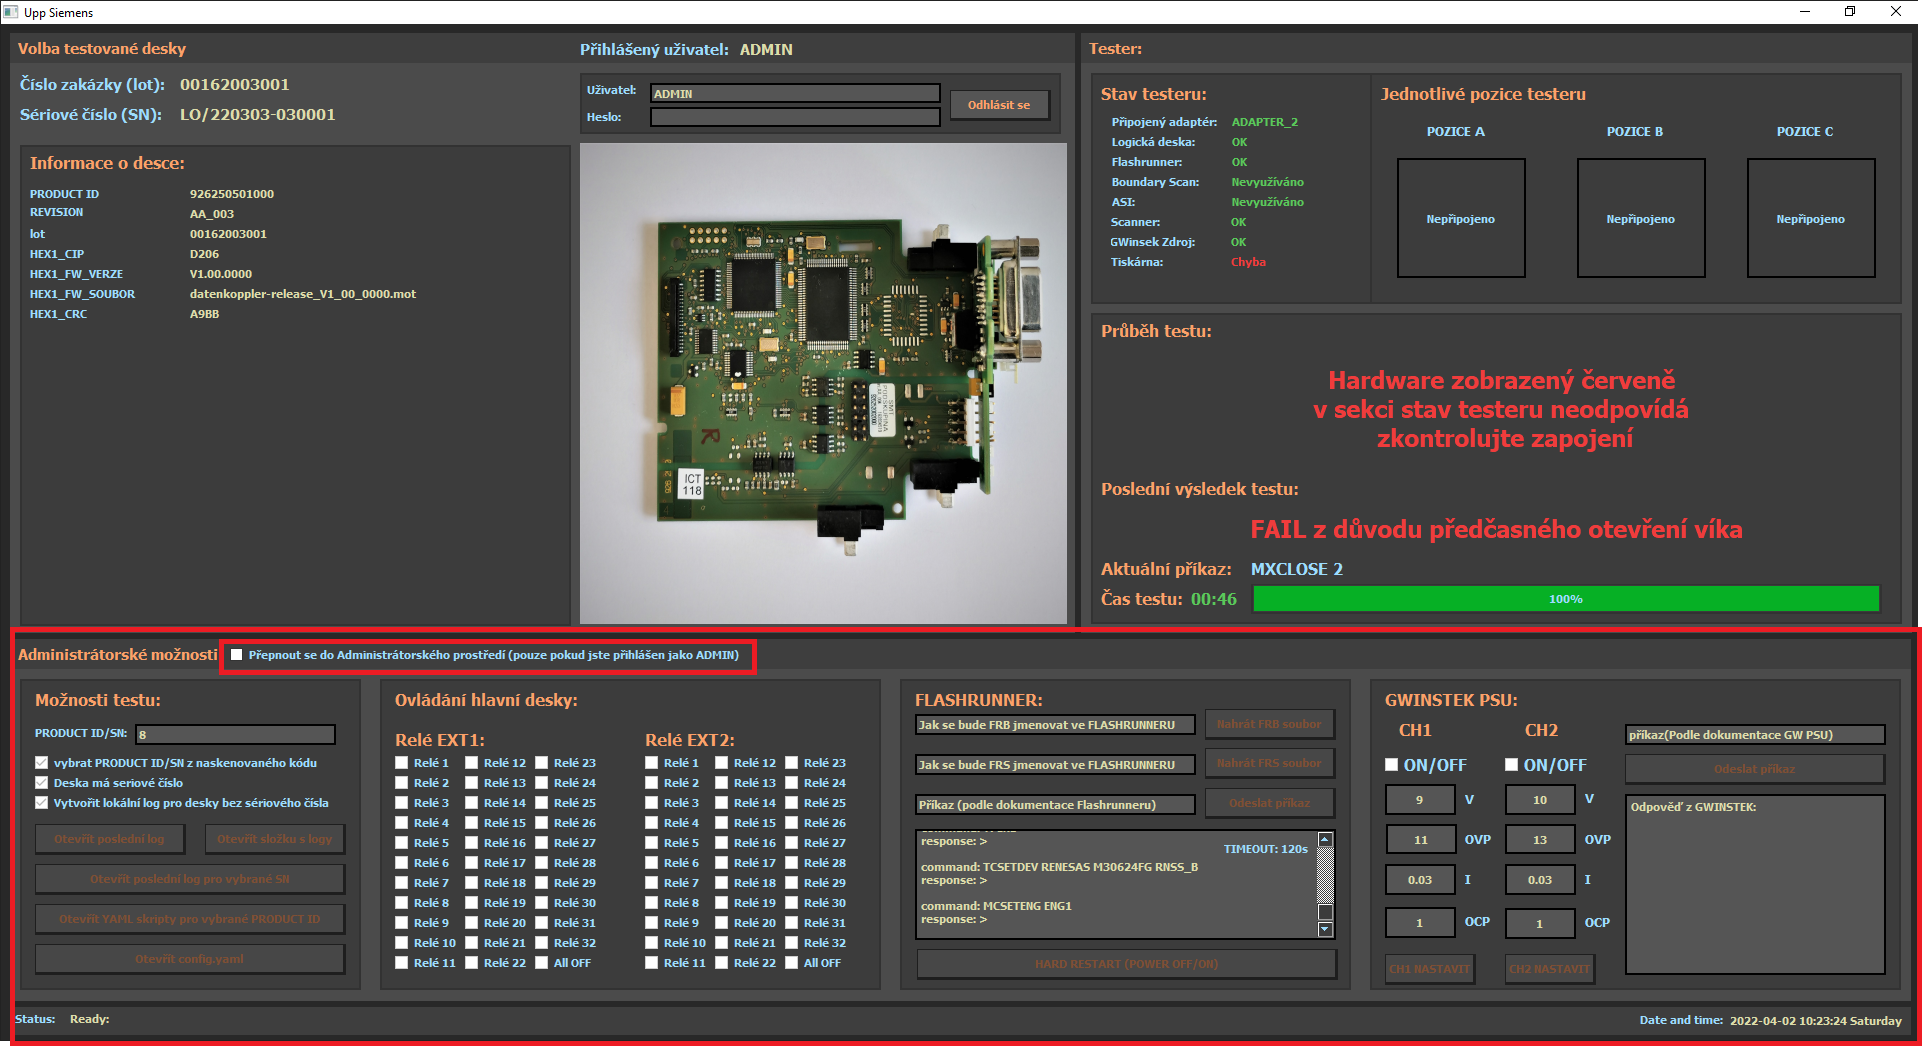
\includegraphics[width = 1\textwidth]{obrazky/ADMIN_edited.png}
    \caption{Odemčení administrátorského prostředí}
\end{figure}




\subsection{Sekce Možnosti testu:}
V případě, že deska nemá sériové číslo,
je zde možné povolit spuštění test bez naskenovaného SN.
Tuto možnost lze aktivovat odškrtnutím políčka "deska má sériové číslo".
Dále jsou zde tlačítka pro snazší otevírání složek a souborů s logy popř.
souborů popsaných v sekci "Struktura složek na konci dokumentu". 


\subsection{Sekce ovládání hlavní desky:}
Zde je možné přepínat jednotlivá relé na relé kartách v právě připojeném ADAPTÉRU.
\textbf{\color{red} NEVHODNÝM PŘEPNUTÍM RELÉ VŠAK MŮŽE DOJÍT K DESTRUKCI NĚKTERÝCH ZAŘÍZENÍ.}
Zapojení Relé karet lze najít ve schématu el. zapojení. 

\subsection{Sekce FLASHRUNNER:}
V této sekci je možné komunikovat s FLASHRUNNEREM pomocí zpráv komunikačního protokolu, který je popsán
v dataseheetu FLASHRUNNERU.
Dále je zde možné odesílat FRB a FRS soubory bez nutnosti vydělávání SD karet.

\subsection{Sekce GWINSTEK PSU:}
V této sekci je možné ovládat programovatelný zdroj GWINSTEK GPP-2323.
Jsou zde přednastaveny pole pro nastavování základních hodnot napětí a proudů.
Pro rozšířené možnosti lze využít pole v pravé části a posílat do programovatelného
zdroje příkazy podle datasheetu pro GWINSTEK GPP-2323

\section{Chyby}
V případě chybových hlášek zobrazených v části 3.
Se zkuste odhlásit odebráním karty a znovu přihlásit.
Po opakovaném přihlášení se může stát, že se zobrazí chybová hláška: ARRIGO neodpovídá.
V tomto případě zkuste počkat 40 až 60 sec. Tester totiž provádí po opětovném přihlášení sebekontrolu,
která může chvíli trvat. Pokud se chybová hláška neodstraní ani po uplynulé čekací době zkusit software restartovat.
V případě, že chybová hláška není odstraněna kontaktujte povolanou osobu. Například chyba z důvodu špatného připojení
tiskárny může vypadat takto:
\begin{figure}[ht!]
	\centering
	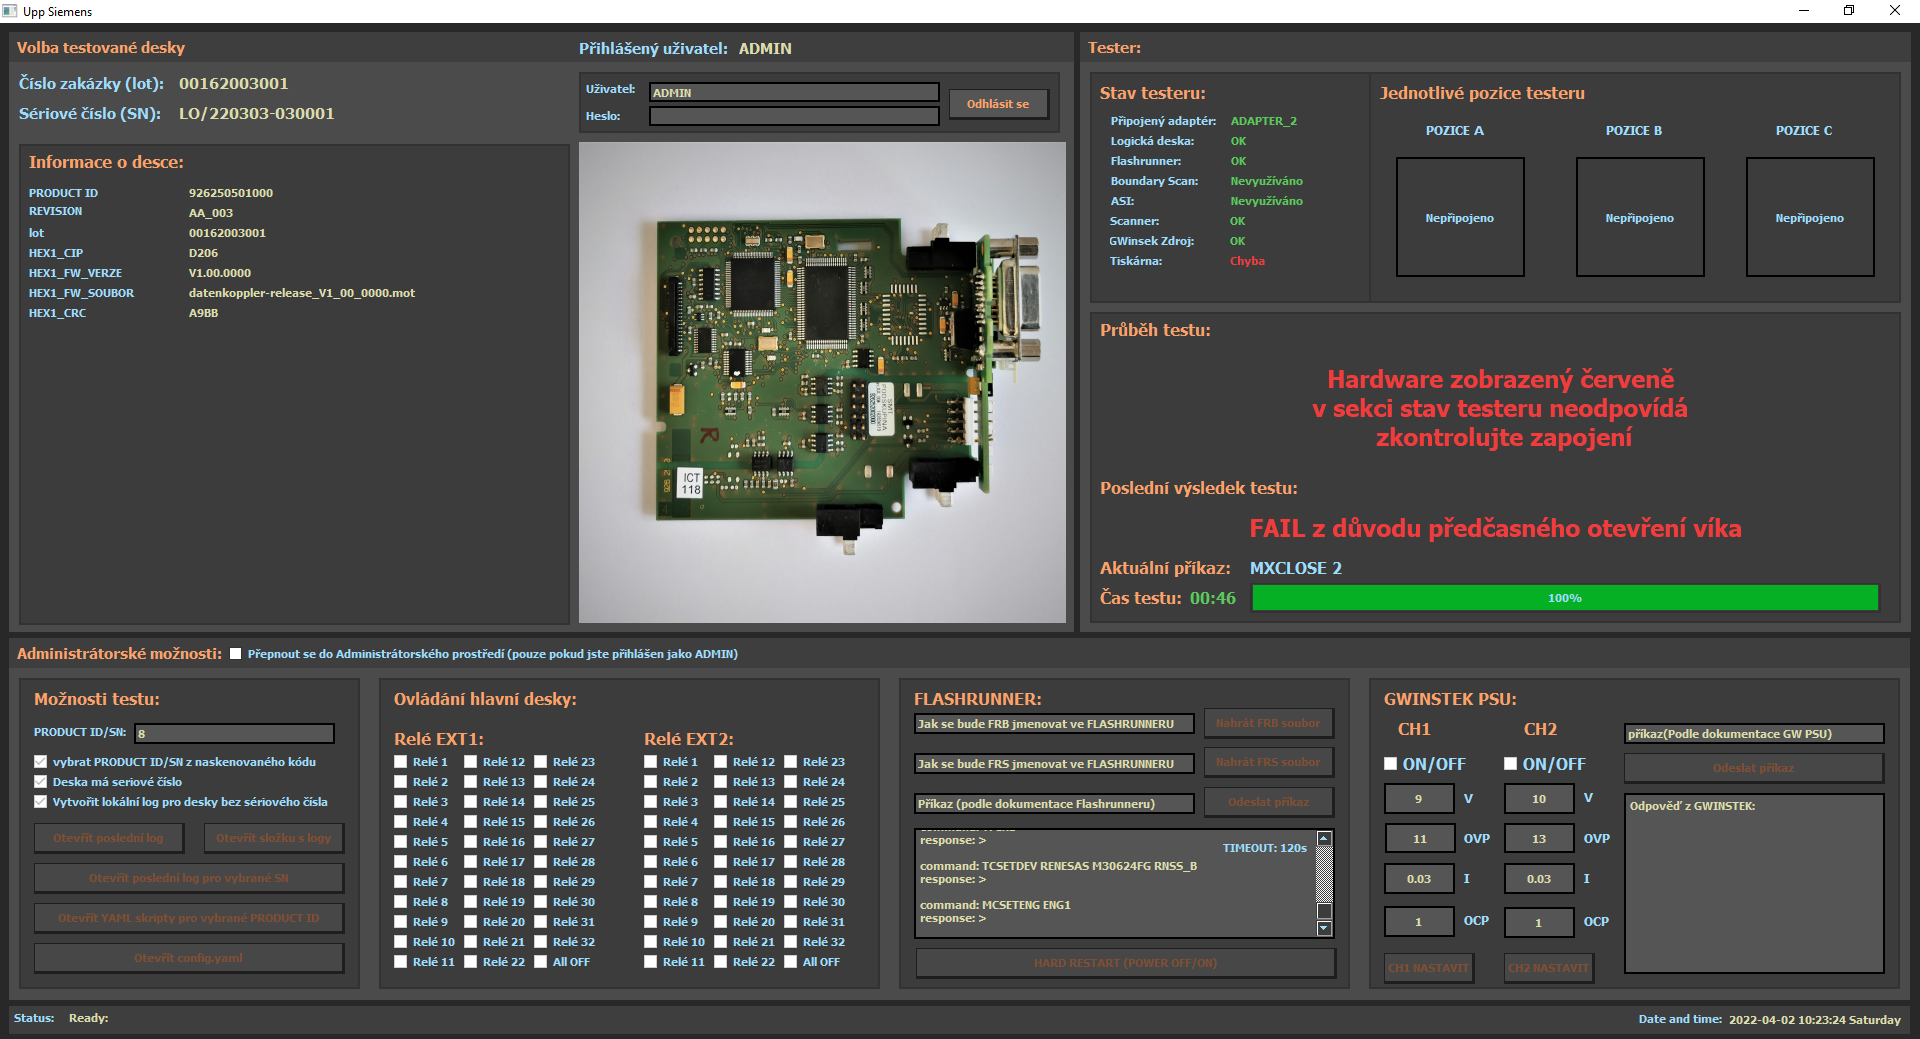
\includegraphics[width = 1\textwidth]{obrazky/HW_FAULT.PNG}
    \caption{chybová hláška z důvodu špatného připojení tiskárny}
\end{figure}



\clearpage
\chapter{Struktura složek:}
SOFTWARE lze konfigurovat pomocí souboru config.yaml.
Zde je možné měnit konfiguraci veškerého připojeného hardwaru, cestu k ukládaným logům,
WSDL k EMES atd.
Tento soubor také obsahuje postup testovacích procedur pro každé DUT v závislosti na "Material Number" s předponou P.
Pro větší přehlednost lze v každém testu volat vnořený yaml script,
který obsahuje skript s příkazy definovanými v datasheetu pro FLASHRUNNER.
Tyto příkazy jsou však upraveny tak, aby odpovídaly syntaxi .yaml souborům
(Obr.\ref{fig:Útržky ze souboru config.yaml}).

\begin{figure}[ht!]
	\centering
	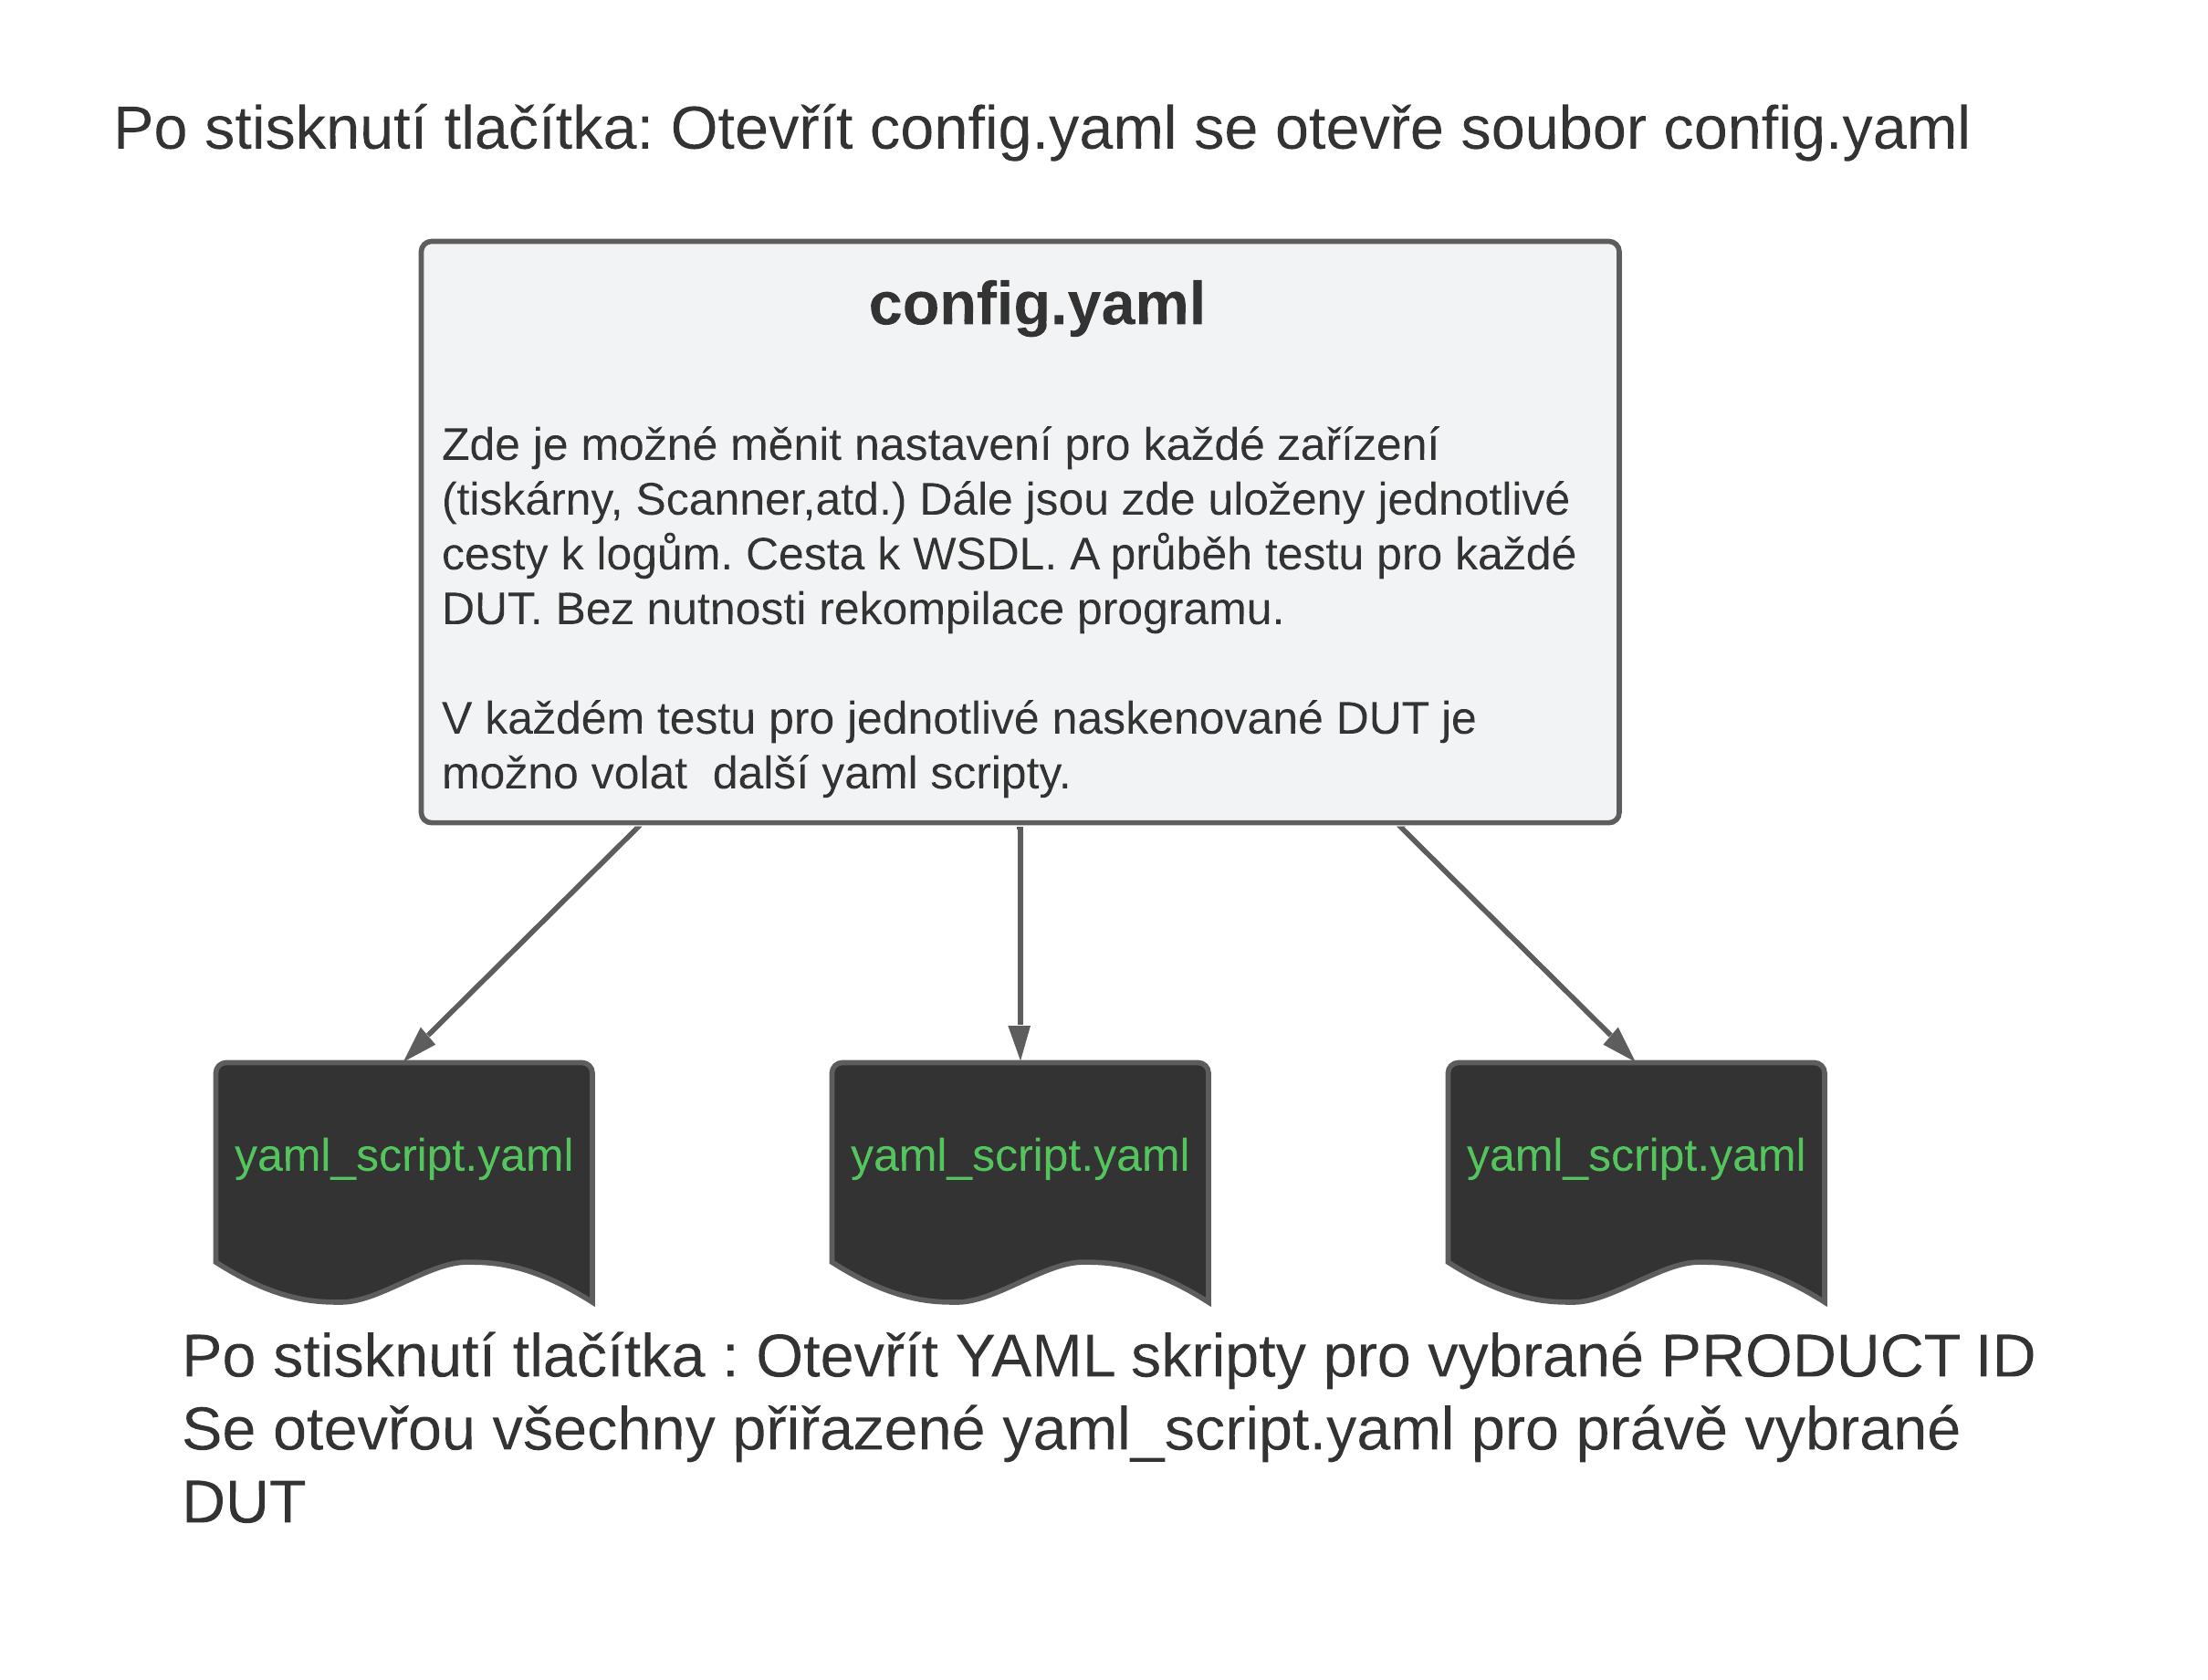
\includegraphics[width = 0.5\textwidth]{obrazky/Folder_diag.png}
    \caption{Struktura složek}
    
\end{figure}

Na následujícím  obrázku jsou útržky ze souboru config.yaml, kde je příklad pro nastavení WSDL a průběhu testu pro DUT,
které má material number 926251703000.
V STEP3 se zavolá script uložený na cestě:\\
\mbox{C:\/Users\/prod\_admin\/Desktop\/UPP\_refactor\/YAML\_SCRIPTS\/926257702000\_ATMEGA325.yaml}.\\
V tomto scriptu jsou dvě části INIT\_FR a MAIN. Tyto části budou volány postupně podle pořadí v jakém jsou napsány v souboru config.yaml. 

\begin{figure}[ht!]
	\centering
	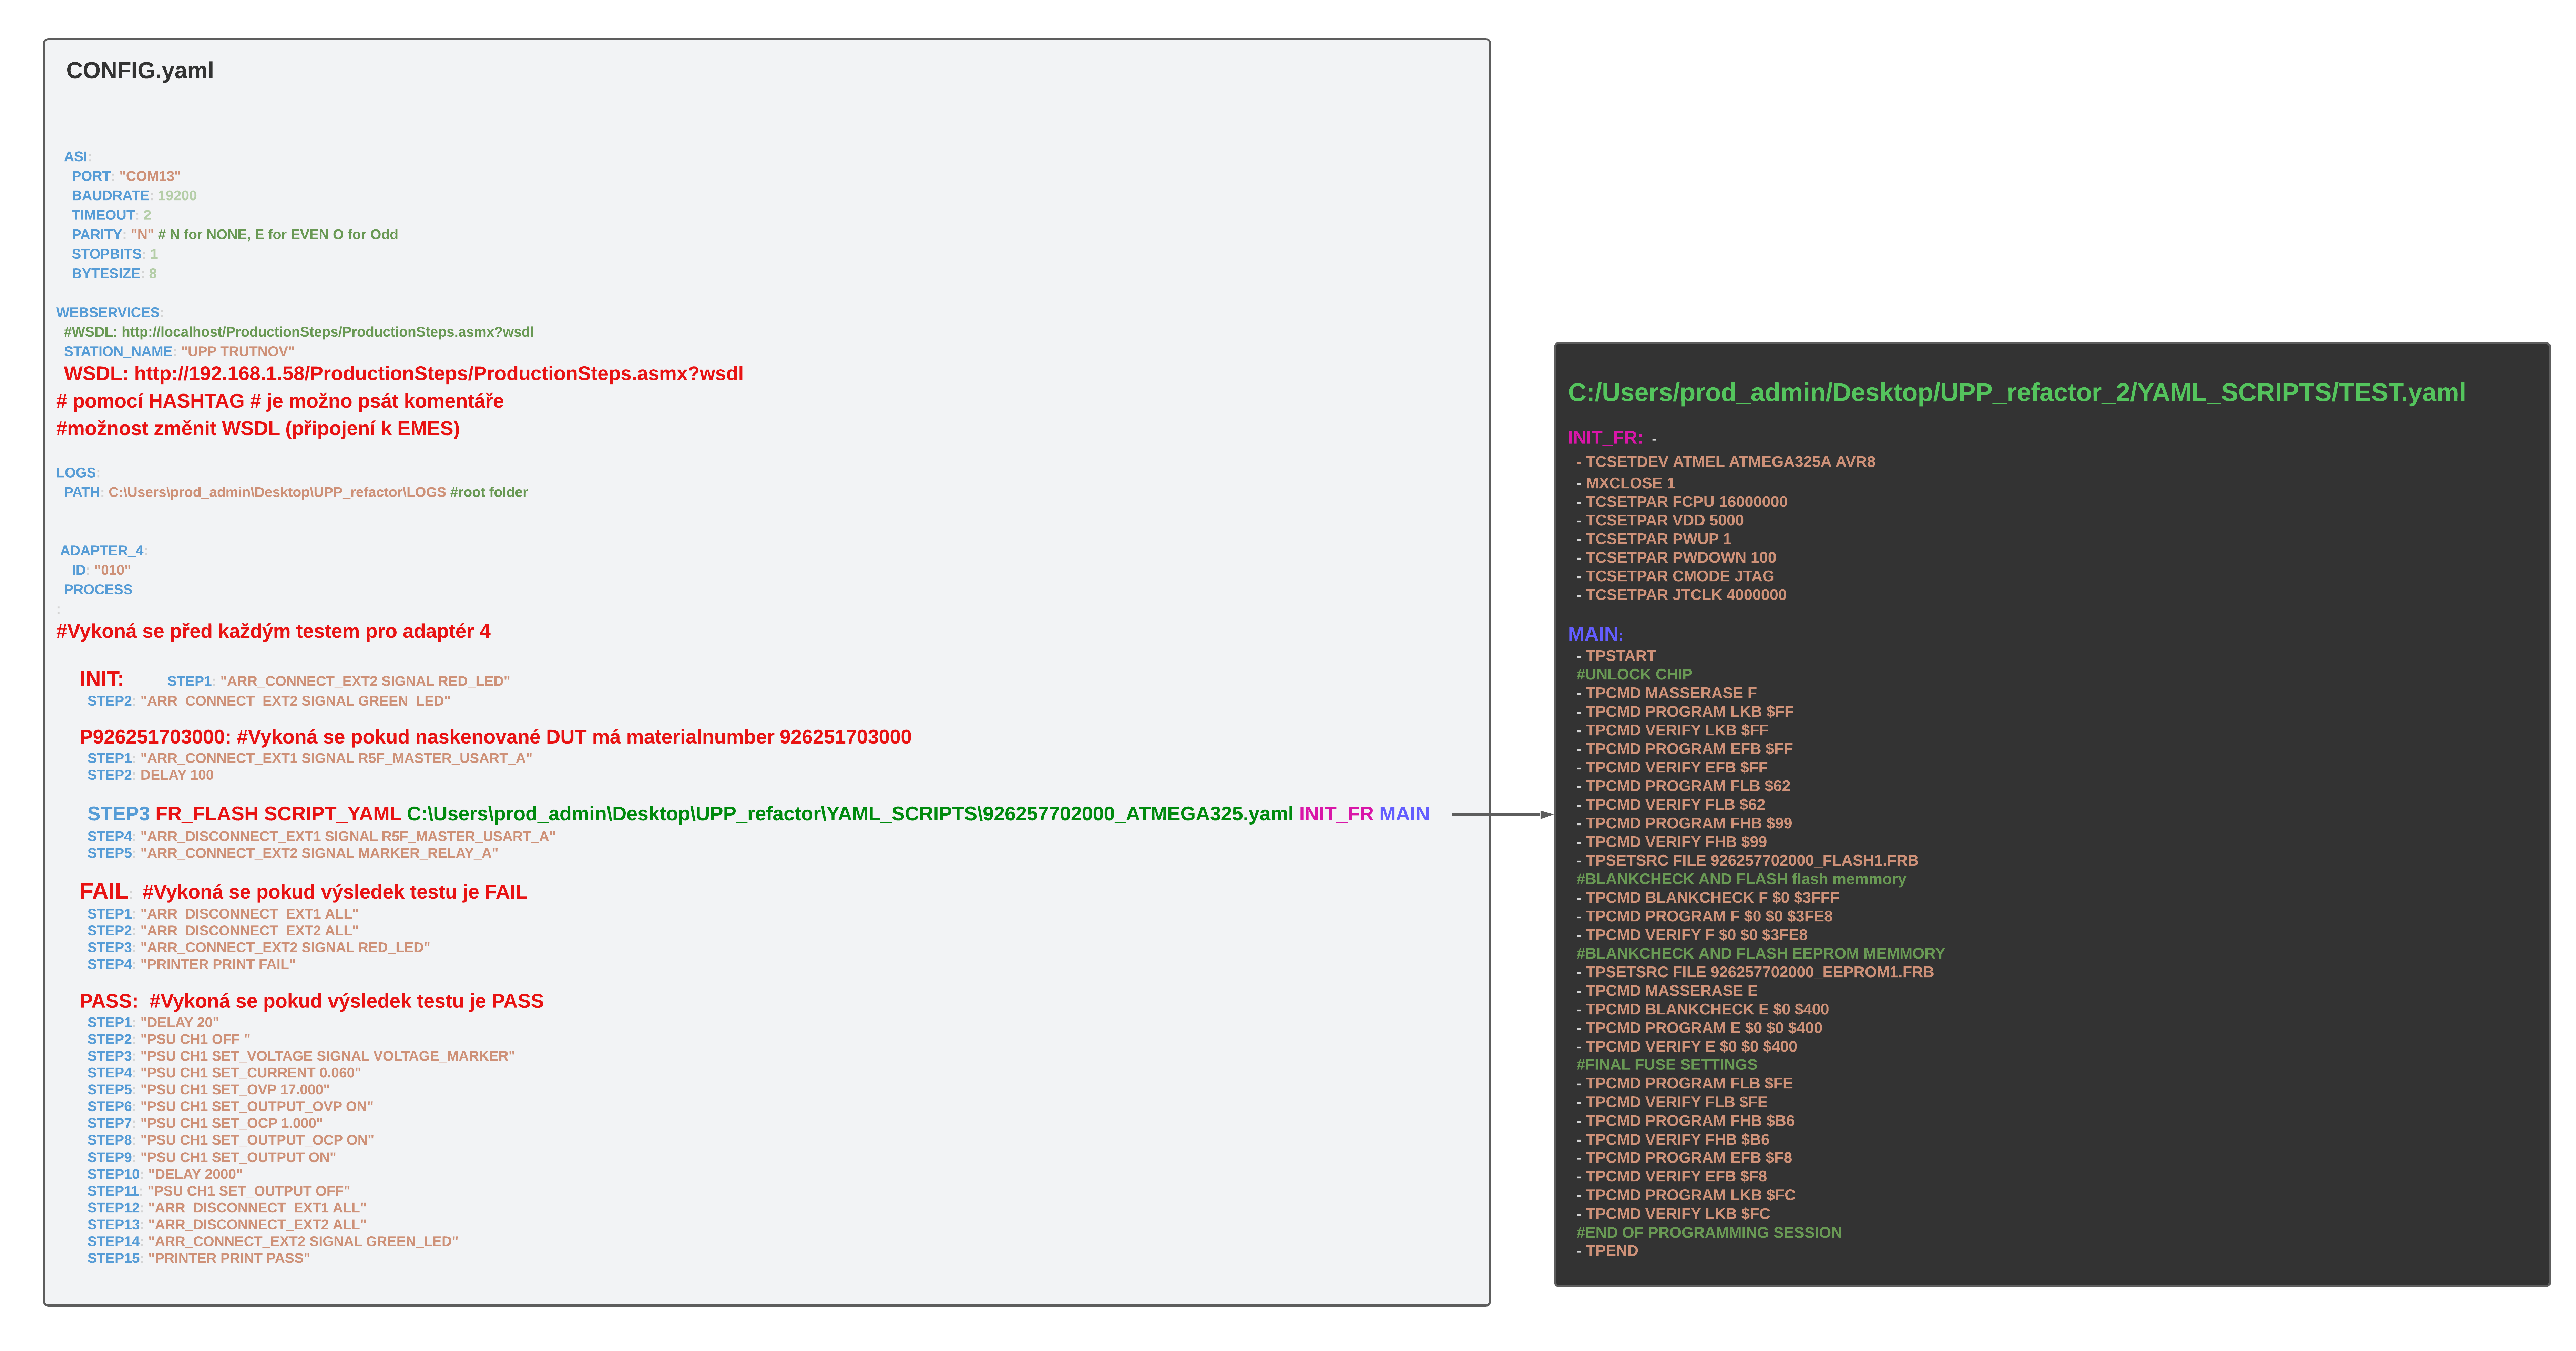
\includegraphics[width = 1\textwidth]{obrazky/FOLDER_TEXT.png}
    \caption{Útržky ze souboru config.yaml}
    \label{fig:Útržky ze souboru config.yaml}
\end{figure}

Je tak možné zavolat například pouze část INIT\_FR smazáním "MAIN"\ ze souboru config.yaml.
Následující příkaz bez volání MAIN sekce z .yaml scriptu by pak vypadal následovně:\\
STEP3: FR\_FLASH C:/.../YAML\_SCRIPTS/926257702000\_ATMEGA325.yaml INIT\_FR

\section{Přídavné utility}
 Softwarový balíček nabízí celou řadu utilit pro snadnější konfiguraci a údržbu testeru.
 Jedná se například o programy umožňující nastavovat správnou syntaxi yaml scriptů, jednodušší procházení logů,
 testování jednotlivých částí testeru bez nutnosti připojení do EMES, přímou komunikaci s programátory,
 ovládání značkovačů (frézek), testování EMES, simulace TCP/IP serveru pro přihlašování pomocí karet, debugování apod.

